\section{Discusi\'on}

\subsection{PageRank}
Claramente podemos notar que a medida que el C crece, el algoritmo toma más iteraciones en achicar la norma. Esto se debe a que el grado de aleatoriedad elimina el peso de la unión entre los sitios e indica una uniformidad en el comportamiento, entonces la matriz si bien estocástica ahora se encuentra distribuida esa suma $=$ 1 por columna en varias filas. Esto produce mayor cantidad de iteraciones en el método de la potencia ya que la mayor uniformidad de la matriz provoca que ninguna 'zona' de la matriz absorba más que las demás.   $[1]$\\
También es bastante notorio que a pesar de que los distintos casos de prueba sean muy diferentes entre si y hasta cientos de veces más grandes, la evolución de la norma converge de formas casi idénticas y lo mismo sucede para las iteraciones requeridas hasta llegar a la norma variando el parámetro c.

\subsection{Análisis cualitativo}

En esta sección procederemos a discutir sobre la calidad de resultados que obtenemos de cada algoritmo y luego los compararemos entre si.\\
Como el objetivo de este trabajo práctico esta enfocado al ranking web que se le asigna a los distintos sitios de internet, consideramos como buenos resultados aquellos que aparecerían en la primer página de los buscadores, es decir, los primero 10 resultados serán los que consideraremos para el análisis.

\subsubsection{PageRank}
Según el paper de Bryan y Leise, quienes proponen el algoritmo, lo más común es que el valor del navegante aleatorio sea de 0.15. Por lo tanto creemos que con este valor es donde aparecerán los mejores resultados, pero también veremos que sucede con valores de 0.5 y 0.85, ya que estos valores indican por un lado que la probabilidad del navegante entre quedarse e irse es equiprobable y por otro lado es el inverso de lo que ellos consideran como el valor más común. En valores de 0 y 1 no tendrían sentido el análisis ya que por un lado daría la matriz original y por el otro una matriz equiprobable.\\
El caso de prueba que utilizaremos es el dado por la cátedra, \textbf{Abortion}, y lo elegimos ya que es un tema bastante discutido donde se pueden encontrar resultados interesantes.

\paragraph{Resultados con un c=0.15}
\begin{enumerate}
\item
http://www.allexperts.com/about.asp\\
AllExperts.com
\item
http://www.nrlc.org\\
National Right to Life Organization
\item
http://www.phone-soft.com/at/cyber-world/international/o1480i.htm\\
PHONE-SOFT INTERNET DIRECTORY INTERNATIONAL:HERB THERAPY LINKS
\item

http://www.lm.com/~jdehullu\\
Ariadne's Thread: On abortion, affirmative action, hate speech
\item


http://www.plannedparenthood.org\\
Planned Parenthood Federation of America
\item

http://www.gynpages.com\\
Abortion Clinics OnLine
\item

http://www.care-net.org/link.htm\\
CareNet Links
\item

http://www.naral.org\\
NARAL: Abortion and Reproductive Rights: Choice For Women
 \item

http://www.crosswalk.com/ftr/1,,17,00.htm \\
Crosswalk.com Forums - Welcome
 \item

http://www.cais.com/agm/main\\
The Abortion Rights Activist Home Page

\end{enumerate}

\paragraph{Resultados con un c=0.5}
 \begin{enumerate}
 \item "http://www.allexperts.com/about.asp\\
AllExperts.com"
 \item"http://www.nrlc.org\\
National Right to Life Organization"
 \item"http://home.about.com\\
About - The Human Internet"
 \item"http://www.phone-soft.com/at/cyber-world/international/o1480i.htm\\
PHONE-SOFT INTERNET DIRECTORY INTERNATIONAL:HERB THERAPY LINKS"
 \item"http://www.lm.com/~jdehullu\\
Ariadne's Thread: On abortion, affirmative action, hate speech"
 \item"http://www.plannedparenthood.org\\
Planned Parenthood Federation of America"
 \item"http://www.care-net.org/link.htm\\
CareNet Links"
 \item"http://www.gynpages.com\\
Abortion Clinics OnLine"
 \item"http://www.marchforlife.org\\
The March For Life Fund Home Page"
 \item"http://www.jbs.org\\
The John Birch Society"
 \end{enumerate}
 
\paragraph{Resultados con un c=0.85}
 \begin{enumerate}

 \item"http://www.jbs.org\\
The John Birch Society"\\
 \end{enumerate}
 
\subsubsection{HITS}
\subsubsection{Indeg}

\subsubsection{Comparación}






\subsection{Ejemplos de comportamiento esperado}

A continuación veremos en redes pequeñas como se comporta el algoritmo para ver si su comportamiento es el esperado.

\subsubsection{HITS}
 \begin{figure}[!htb]
\begin{center}
    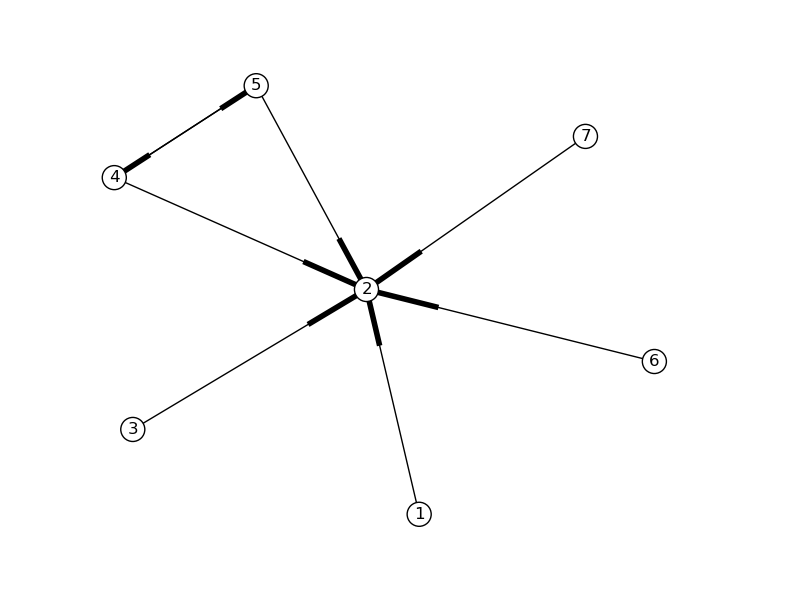
\includegraphics[scale=0.5]{imagenes/test4.png}
    \caption{Red de 7 nodos}
    \end{center}
\end{figure}

Resultado obtenido:
   $$ 
\begin{bmatrix}
              &    Autoridad  &  Hub \\
 Nodo 1 &   0.000000    &      0.383092       \\
 Nodo 2   &  0.967054    &  0.000000     \\
 Nodo 3   &  0.000000   &     0.383092  \\
 Nodo 4   &  0.180008    &     0.454401       \\
 Nodo 5   &  0.180008    &     0.454401        \\
 Nodo 6   &  0.000000    &      0.383092     \\
 Nodo 7   &  0.000000   &     0.383092 \\
\end{bmatrix} 
$$

Efectivamente podemos observar que en la columna de autoridades el nodo 2 es el mayor ya que es el que mas apuntado esta y todos aquellos que tienen 0 es porque no son apuntados por ninguno. Por otro lado en la columna de hubs podemos ver que los nodos 4 y 5 son los que mayor valor tienen ya que son los que mas apuntan a otros nodos con 2 salidas.
